\chapter{Development}
To extend the HyperANF algorithm, we will use the HyperANF implementation in HyperBall. Initially, the algorithm takes an existing non-empty directed graph as input. This graph can be seen as static and therefore HyperANF can perform a complete calculation on it. After HyperANF is complete, the calculated counters can be used as the initial counters for the dynamic algorithm. For every insertion and deletion in the dynamic graph, these counters are manipulated. If an edge is added, nodes might reach more  nodes and their counters should be raised. Similarly for deletions, if an edge is deleted, nodes might reach fewer nodes and their counters should be decreased.

\section{Preliminaries}

\subsection{Dynamic graphs}

To achieve a dynamic graph, the ability to insert new nodes and edges (called entries in this section) to an existing graph is needed. The graph files used by HyperANF are tightly compressed in a byte stream, which makes it an expensive operation to modify the graph at an arbitrary point. This makes it infeasible to insert every additional entry directly into the graph file. Instead, new entries can be stored in some other data structure.

The additional entries can either be stored in a high-level data structure or a byte stream. Keeping them in a high-level data structure will consume a significant amount of storage already at a low number of extra entries. A high-level data structure takes up more memory as each number is always the same size, no matter what the value is. For example, the value 3 can be expressed by two bits but a high level integer always take a fixed amount of bits to express it.  Additionally, if each node has a structure containing the neighbors, a significant amount of space will be used by the pointers to those structures. 

If a byte stream is used, the same problem as the original one occurs. Even though this byte stream will be smaller, there will be a point where it is unreasonable to resize the stream and reposition the existing entries at each new entry. Regardless of which method is used, the extra entries and the original graph eventually have to be merged.

\subsubsection{Merging two graphs with webgraph}
The webgraph framework has a method for creating a new graph $G$ by taking the union of two subgraphs $G_1$ and $G_2$. The graph $G$ works by simultaneously reading from both streams $G_1$ and $G_2$ to produce the nodes and their neighbors. The sub graphs can be unions of other graphs as well. This means that an arbitrary number of graphs can be joined using this method. However, having lots of recursive unions create a large overhead in time when fetching nodes and edges \cite{webgraph}. 

The framework also supports storing a union-graph to disk. This removes the overhead of any union. As the graph express some arcs by references to previous arcs, storing is slow. Ignoring the references makes the graphs larger but it increases the running time of the storeing step.

\subsubsection{Memory dependent merging}
To leverage the benefits of both high level structures and byte streams, we use a mixture of both to achieve dynamic graphs. The original graph is kept as a byte buffer and the additional entries are saved in a high level structure. The high level structure was chosen as additions are faster than in a byte stream graph. We prioritize fast edge additions as the addition time has a larger impact on the overall performance than the iteration time (see Section \ref{bench:graphStructure}). Each new bulk of edges is inserted into the high level structure. The union method of webgraph can then be used to union the high level structure and the original graph, creating a dynamic graph.

The overhead of recursive unions can be avoided by limiting the number of unions to one. By inserting each bulk insertion into the same high level structure, and keeping the original graph separated, the current union can be replaced by a new one. However, the problem of high memory overhead when using a high level structure still remains. Our solution is to merge the graphs when the additional entries' memory usage, compared to the byte stream graph, reaches a certain ratio. At this time, the unioned graph is stored to disk. The graph is then loaded as a byte stream and the additional edges become part of the original graph. This resets the memory overhead of the high level data structure. Both the time and memory usage of this technique are nearly optimal (see Section \ref{bench:unionVsStored}).

\subsection{HyperLogLog resizing}
After new nodes are added to the graph, new counters have to be created for them. The initial counters retrieved by HyperANF are represented as an array of 64-bit numbers. This representation is kept unchanged as it minimizes the amount of wasted space usage. It also minimizes the number of objects created on the heap. However, as new counters are needed, the array must be resized. We use a geometric expansion which gives $O(1)$ amortized time per insertion \cite{dynamicarrays}. Amortized time is the average time spent on each operation. Geometric expansion means that when an element cannot fit the array, the length of the array is increased by a factor. This is how the standard implementation of ArrayList in Java performs dynamic increase. A larger factor implies a small average number of copies per inserted element, but a high amount of unused space. The amortized number of copies per inserted element for a factor $r$ is roughly $\frac{1}{(r-1)}$ and the average unused space is $\log(r)*\frac{r}{(r-1)} - 1$ \cite{dynamicarrays}.

Under the assumption that the graph expands slowly relative to its size, resizing events will be sparse and a large factor implies a large amount of unused memory. Therefore, it is more beneficial to let the array increase by a small factor. With the factor $r = 1.1$, an average of $4.8$\% space is unused and every element will on average be copied $10$ times.

\section{DANF: The first attempt}

The following non-optimized version of DANF is the intuition of the algorithm. It will be refered to as the two-BFS algorithm. The two main phases of our algorithm, the collecting BFS and the propagation BFS, are introduced. 

After an edge is added to the graph, we update the HyperLogLog counters of all nodes affected by insertion. Figure \ref{fig:collect_and_propagate} is used as an example. The thin arrows are the edges. The circles are the nodes included in the counters produced by the collection step. The bold arrows represent the propagation step. Let $e = (2,4)$ be an edge added to the graph. The data with all the nodes reachable from $4$ has to be propagated to the nodes that can now reach $4$ via $2$. This is performed in two phases: collecting BFS and propagating BFS.

The collecting BFS is responsible for creating a HyperLogLog counter for each level in the search and add all nodes in the frontier to the counter. The collecting BFS is performed from the to node of the added edge. The nodes included in each level's HyperLogLog counter are visualized as the circles in Figure \ref{fig:collect_and_propagate}. These counters represents all nodes that $4$ reaches in $l_4$ steps. The collecting BFS stops at level $h-1$ and returns an $h$-long list of counters. The $h$'th step is not needed as not even $2$ can reach level $h$.

The propagating BFS is responsible for updating the counters of all nodes that now reach $4$, as they might have been changed by the insertion. To find all nodes that can reach $4$, a BFS is performed from $2$ in the transpose of the graph. For every level $l_2$ in the BFS, the frontier of nodes in the BFS can reach all nodes that the collecting BFS reached in $h-1-l_2$ steps. To update the counters of the nodes at level $l_2$, the current counters of the nodes are merged with the counters from collecting steps $l_4 \leq h-1-l_2$ retrieved in the collecting BFS. The propagation BFS stops after $h-1$ steps, when all affected node counters are updated.

After the two-BFS algorithm has completed an update in the graph, the collected counters are thrown away as they might be different in the next update.

We will now prove the correctness of the two-BFS algorithm:

\begin{figure}[h]
\centering
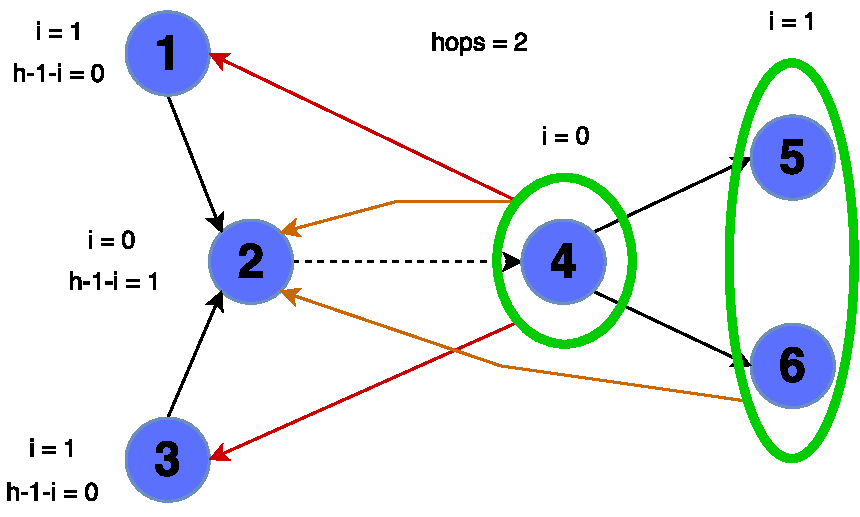
\includegraphics[]{trivial_collect_and_propagate}    
\captionsetup{justification=centering}
\caption {Visualization of the collect and propagate steps}
\label{fig:collect_and_propagate}
\end{figure}


\begin{theorem} Given that the two-BFS algorithm and HyperANF use the same hashing function, the two-BFS algorithm yields node counters identical to a HyperANF recalculation.

\begin{proof}Let $S_\text{alg}(v)_i$ for $alg \in \{\text{2bfs}, \text{hanf}\}$ be the set of nodes that the algorithm "alg" includes in the counter of $v$ after $i$ edges have been inserted. Let $N_\text{alg}(v)_i = S_\text{alg}(v)_i \backslash S_\text{alg}(v)_{i-1}$.\\

\noindent\textit{Base case:} $i = 0)$ As the algorithm uses HyperANF to calculate the initial counters, $S_\text{2bfs}(v)_0 = S_\text{hanf}(v)_0$.\\

\noindent\textit{Inductive hypothesis: } $\forall i \leq n : S_\text{2bfs}(v)_i = S_\text{hanf}(v)_i$.\\

\noindent\textit{Inductive case: } $n + 1)$  $S_\text{hanf}(v)_{n+1} = \{ u : dist(v,u) \leq h \}$ and $S_\text{2bfs}(v)_{n+1} = S_\text{2bfs}(v)_{n} \cup N_\text{2bfs}(v)_{n+1}$. Let the added edge be $e = (v,u)$. In the propagation step at a node $z$ of depth $dist(z,v)$ all counters from the collecting step of depth $\leq h-1-dist(z,v)$ will be unioned with the counter of $z$. As $z$ is $dist(z,v)$ steps away from $v$, $dist(z,u) = dist(z,v) + 1$. This means that $z$ can reach $h-(1+dist(z,v))$ steps into the newly reachable nodes. So $z$ will get all new nodes $\leq h$ steps away, hence $N_\text{2bfs}(v)_{n+1} = N_\text{hanf}(v)_{n+1}$. By the inductive hypothesis: $S_\text{2bfs}(v)_{n+1} = S_\text{2bfs}(v)_n \cup N_\text{2bfs}(v)_{n+1} = S_\text{hanf}(v)_n \cup N_\text{hanf}(v)_{n+1} = S_\text{hanf}(v)_{n+1}$. As both algorithms use the same hashing function, and the same nodes are included in the counters, the resulting node counters will be identical.

\end{proof}
\end{theorem}

\section{Optimized Breadth-first search}

A problem with the two-BFS algorithm described above is that it only supports single insertions at a time. By bulking the edges, several BFS's can be performed at the same time to speed up the insertion time. 

The algorithm MS-BFS \cite{msbfs} does several BFSs at the same time very effectively. MS-BFS is magnitudes faster than a parallel standard BFS implementation and hence will be used in the algorithm. 

\subsection{Visitors}
In order to prune paths in the BFS, there needs to be a way to stop the individual BFSs. We developed a method to pass to the MS-BFS a visitor function (not related to the common Visitor design pattern). The visitor will be called every time a group of BFSs reach a node. The group of BFSs reaching the visited node is represented by a list of bits and is passed to the visitor. If the visitor wants to stop the propagation of a BFS from this node it can clear the corresponding bit. No modifications to the algorithm needs to be done, other than adding the visitors, as MS-BFS already use a list of bits to propagate the BFSs.

\subsection{Travelers}
We developed a new concept called travelers. The purpose of the traveler is to bring data along with BFSs which is passed to the visitors. This removes the need to loop through which source nodes reached the visited node. Travelers have to be able to merge when several BFSs reach a node to avoid increasing the space complexity of the algorithm. 

\subsection{Extended algorithm}

The extended algorithm is presented in Figure \ref{fig:extended_ms-bfs_algorithm}. It has only slight modifications compared to the algorithm in section 4.1.1 from \cite{msbfs}. The visitor is called on line 16. The neighbors are not inspected if the visitor returns an empty set. The travelers are merged at lines 19 to 22. If the neighbor will be visited from other nodes, i.e. the $visitNext$ bits are not empty, the neighbor's traveler is merged with the traveler from the current node.

\begin{figure}[h]
    \begin{lstlisting}[mathescape]
Input: $G = (N,E)$ a graph containing $N$ nodes with edges $E$
       $S$ = BFS source nodes
       $V$ = Visitor function
       $T$ = Travelers
for each $s_i \in S$
    $seen[ s_i ] \leftarrow 1 << i$
    $visit[ s_i ] \leftarrow 1 << i$
for each $t_i \in T$
    $travelers[s_i] \leftarrow t_i $
reset $visitNext$
reset $travelersNext$

while $visit \neq \emptyset$
    for $i = 1, ... , N$
        if $visit[i] = \emptyset$, skip
        $visit[i] \leftarrow V(i,visit[i],travelers[i])$
        if $visit[i] = \emptyset$, skip
        for each $n$ where $(i,n) \in E$
            $traveler \leftarrow travelers[i]$
            if $visitNext[n] \neq \emptyset$
                $traveler \leftarrow traveler.merge(travelersNext[n])$
            $travelersNext[n] \leftarrow traveler$
            $visitNext[n] \leftarrow visitNext[n]$ $|$ $visit[i]$

    for $i = 1, ... , N$
        if $visitNext[i] = \emptyset$, skip
        $visitNext[i] \leftarrow visitNext[i]$ $\& \sim seen[i]$
        $seen[i] \leftarrow seen[i]$ $|$ $visitNext[i]$
    $visit \leftarrow visitNext$
    reset $visitNext$
    $travelers \leftarrow travelersNext$
    reset $travelersNext$
    \end{lstlisting}
    \caption{Extended MS-BFS algorithm in pseudo-code}
    \label{fig:extended_ms-bfs_algorithm}
\end{figure}


\section{DANF: The final algorithm}
\subsection{Node history}

MS-BFS speeds up the algorithm significantly, but further optimizations can be done to the individual BFSs. To update a counter, the algorithm has to do two BFSs for every edge added. A large portion of the time spent by the algorithm will be consumed by these BFSs. Therefore, the ability to prune BFSs early implies significant time improvement. So far, the collecting BFS must traverse the graph $h$ steps to gather all data needed. This is because every node only keeps track of its registers, resulted by a search in $h$ steps. If all nodes also keep track of their registers in $h-1$ steps, then the collecting BFS need to traverse $h-1$ steps. This as in the $h-1$'st step, the collecting BFS can use the $h-1$ history of all nodes to calculate the $h$'th step. For every extra history level added, the collecting BFS can stop one step earlier. By saving every history level of all nodes, the collecting BFS only needs to visit the immediate neighbors of a new node $v$ to be able to calculate the HyperLogLog counter of $v$. 

During the HyperANF phase of the algorithm, the intermediate counters in HyperANF can be used to calculate all history levels of all nodes. HyperANF works in iterations. During the $i$'th synchronization, the counters will represent the $i$'th level of all nodes' history. So, instead of only using the last level from HyperANF, we save all levels. The $h$'th level we refer to as the top counter and level $0$ to $(h-1)$ as history counters. All levels combined will be referred to as counter collection.  

Now, every node has its history which has to be updated with every edge update. For an edge $e = (u,v)$ inserted, the collecting BFS has to gather the node history from all neighbors of $v$ and union them into one. Then, the propagation BFS has to propagate this history in the transpose of the graph. 

With node history, the algorithm has $O(hn \log \log n)$ space complexity, as the top counter uses $O(n \log \log n)$ and the history counters use $O((h-1)n \log \log n)$. To insert an edge $e = (u,v)$, the two previous BFSs use $O(2m)$ operations but with node history the collecting BFS uses $O(hd^+(v))$ operations, where $d^+(v)$ is the out degree of node $v$. It is dependent on $h$ as it has to take the union of each history counter. The time complexity of the node history version is then $O(m + hd^+(v))$. In practice, this means a large improvement as it often holds that $hd^+(v) << m$.

Node history speeds up the algorithm but also uses extra space that, for large graphs, can be quite extensive. To create an algorithm that balances the gained speed versus the extra memory usage, the history can be saved for only a subset of nodes. These nodes should be chosen so that as few nodes as possible need to save their history while keeping the BFS distance as short as possible. The algorithm to determine these nodes has to be very fast to avoid affecting the running time of the overall algorithm. Moreover, it has to be dynamic in order to continuously determine the nodes included in the set.

\subsubsection{Vertex cover}
\label{sec:vertex_cover}
We realized that saving the history of the nodes that are in a vertex cover $(VC)$ can significantly improve space usage, yet the BFS can still be bounded by at most two steps.

The top counter still needs to contain counters for all nodes, so that the space complexity of the top counter remains $O(n\log \log n)$. As the history counters only consist of counters of nodes in the $VC$, the history counters' space complexity is reduced from $O((h-1)n \log \log n)$ to $O((h-1)|VC| \log \log n)$. In total, the node history uses $O(((h-1)|VC| + n )\log \log n)$ space.

The trick here is that for all nodes $u$, it holds that: $u \in VC \vee \forall e = (u,v) : v \in VC$. Then, when the collecting BFS searches from a node $v$ it will take at most one step for nodes not in the vertex cover and two steps for nodes in the vertex cover until they reach a frontier of only nodes in the vertex cover. From this frontier, the collecting BFS can calculate $v$'s history and counter by merging the frontier's node histories. The collecting BFS is now bounded by two steps, resulting in $O(d^+(v) + \sum_{u \in s(v)}{d^+(u)})$ operations, where $s(v)$ is the set of neighbors of $v$.

\paragraph{Dynamic minimum vertex cover} \mbox{} \\
At all times, we need to keep track of which nodes are in the vertex cover. This requires a fully dynamic minimum vertex cover algorithm. However, as the minimum vertex cover problem is NP-complete, approximation algorithms must be used. The choice of fully dynamic approximate minimum vertex cover algorithm depends on the ratio between the number of insertions and deletions. A simple greedy algorithm can maintain a $2$-approximation in $O(1)$ time per insertion and $O(n)$ time per deletion \cite{2appdynvc}, while another algorithm that partitions the nodes can maintain the same approximation in $O(\log n )$ amortized time per insertion and deletion \cite{2appdynvclogn}. In our case, deletions will be very sparse in the data stream, which is why we chose greedy algorithm. The greedy algorithm also have the property that if a deleted edge was not in the maximal matching previously, it deletes the edge in $O(1)$ operations. For dense graphs, only a small amount of the edges will be in the maximal matching, which makes the greedy algorithm perform quickly in deletions as well. In practice, the greedy algorithm performs $30,000,000$ edge insertions per second and $5,000,000$ edge deletions per second (see Section \ref{bench:dvc}).
 
\paragraph{Directed graphs} \mbox{} \\
As the standard minimum vertex cover problem is defined for undirected graphs we have to slightly modify the problem for directed ones. The new problem description is as follows; given a directed graph $G = (V,E)$, select a minimum cardinality subset $V' \subseteq V$ such that for all edges $e = (u,v) \in E, u \in V' \vee v \in V'$. The problem is still NP-complete as undirected graphs are a special case of directed graphs. 

By the same reasoning as in the undirected case, a maximal matching is a $2$-approximation of the generalized problem. The greedy algorithm needs to be modified to support directed edges. The only case affected is when an edge in the maximal matching is deleted. Let $e = (u,v)$ be a deleted edge. Previously, the algorithm removed both $u$ and $v$ from the vertex cover and then scanned the outgoing edges from $u$ and $v$ for edges uncovered due to the removal. With directed edges, both incoming and outgoing edges must be verified. This is solved by scanning the outgoing edges of $u$ and $v$ in both the original graph and the transpose of it. The original graph will give the outgoing edges of $u$ and $v$ and its transpose the incoming ones.


\subsection{Edge insertion}

Edge insertion in DANF is now divided into four steps. The first step is checking if a new edge contains any new nodes. New nodes are added to the graph and the top counter is, if necessary, resized to fit new counters of the new nodes. The second step is to check if any new node needs to be added into the vertex cover. For all new nodes in the vertex cover, memory is allocated in the history counters. The third step is calculating the history of the nodes added to the vertex cover. Lastly, the new history is propagated with a BFS in the transpose of the graph to update the counters of the nodes affected by insertion. After these four steps all nodes will have an approximate neighborhood function in their top counters and all nodes in the vertex cover will have their history counters updated. 

\subsubsection{Partial history calculation}
When a bulk of edges is inserted, the vertex cover needs to be modified and the history counters updated. Using a maximal matching \cite{2appdynvc}, which does not delete any nodes upon insertion, the collecting BFS can generate the partial history by searching at most one level. For every node added to the vertex cover, the collecting BFS only needs to retrieve the history of the node before the current bulk insertion. The remaining of the node history will be propagated by the propagating BFS.

The collecting BFS of node $v$ looks through all its neighbors that are in the vertex cover and adds their history to its own. For this, only $O(d^+(v))$ operations are needed, which is an improvement to the time complexity stated in \ref{sec:vertex_cover}. \\


\subsubsection{History propagation}

When a new edge $e = (u,v)$ is added to the graph, many nodes that have a path to $u$ will contain outdated history. The algorithm works by propagating the history of $v$ through the transpose of the graph. If $v$ is not in the vertex cover, the history needs to be calculated from the neighbor nodes. The algorithm is presented in pseudo code (see Figure \ref{fig:history_propagation_algorithm}).

\begin{figure}[h]
    \begin{lstlisting}[mathescape]
e = (u,v) //Edge to add
if(isInVertexCover(v))
    H$_v$ = H(v);
else
    H$_v$ = union of the history of the neighbor nodes;
In BFS; source: u, current node: z, at depth: d{
    d = d+1;  // The BFS is performed from u so the actual depth 
              // (from v) is one higher
    if(isInVertexCover(z)){
        foreach 0 $\leq$ i $<$ h+1-d{
            H(z,i+d).union(H$_v$(i));
        }
    }else{
        H(z,h).union(H$_v$(h-d));
    }
}
    \end{lstlisting}
    \caption{History propagation in pseudo-code}
    \label{fig:history_propagation_algorithm}
\end{figure}

To speed up the algorithm, it needs to be modified to handle several edges at once. In this case, the traveler support of the MS-BFS algorithm can be used. This means that the data provided by the traveler can be used instead of looping through all the source nodes. The travelers will contain the counter registers of their respective source node. When the travelers merge they can take the union of their registers. Also They only need to keep the $h+1-depth$ top-most counters as the others will not reach further anyway. In the visitor the data from the traveler is joined with the existing counters of the visited nodes. The merge function for the traveler is constructed as in Figure \ref{fig:history_propagation_traveler}.

\begin{figure}[h]
    \begin{lstlisting}[mathescape]
Input: t1,t2 = travelers to merge (HyperLogLog counters)
       d = depth of the BFS
Output: a new traveler
tOut = t1.clone
foreach 0 $\leq$ i $<$ h+1-d{
    tOut$_i$ = tOut$_i \cup $t2$_i$
}
return tOut
    \end{lstlisting}
    \caption{History propagation traveler in pseudo-code}
    \label{fig:history_propagation_traveler}
\end{figure}

The visitors have to be slightly modified to make use of this traveler. The only difference is that a visitor uses the counter history from a traveler data instead of taking it from the source nodes.

Given that the partial history calculation makes sure that all nodes in the vertex cover have the history they had before the current insertion, we prove that all nodes  have the correct history after the propagation step: \\

\begin{theorem} Given that HyperANF and DANF uses the same hashing function; after every bulk insertion, all nodes have had all reachable nodes added to their counters. \\\\
\normalfont{To prove this we first need to establish two lemmas:}\\

\begin{lemma} Assume that the history of all the nodes in the vertex cover in bulk insertion $p$ have had all reachable nodes added to their counters after bulk insertion $p$. Then, during bulk insertion $p+1$, only one BFS step is needed to collect the history that any node $v$ would have after bulk insertion $p$. \\\label{lemma:partial_history_calculation}

\begin{proof} Given a node $v$ whose history should be calculated for bulk insertion $p+1$:\\

\noindent\textit{Fact:} It holds that $v \in VC \vee \forall e = (v,u) : u \in VC$.

\noindent Let $N_p(v,h) = \{v\}\bigcup\limits_{u \in s_p(v)} N_p(u,h-1) $ be the reachable nodes of $v$ between insertion $p$ and $p+1$, where $s_p(v)$ is the set of successors of $v$ in step $p$. Let $H_p(v,h) = \{v\}\cup\bigcup\limits_{u\in s_{p}(v)}N_{p-1}(u,h-1)$ be the nodes included in the calculated counter. Let $n_p(v)=s_p(v)\backslash s_{p-1}(v)$.\\


\noindent As no edges are removed: 
$s_p(v) \subseteq s_{p+1}(v)$.\\ 
$H_{p+1}(v,h) = \{v\}\bigcup\limits_{u\in s_{p+1}(v)}N_{p}(u,h-1) = \{v\}\bigcup\limits_{u\in s_{p}(v)}(N_{p}(u,h-1)) \bigcup\limits_{u\in n_{p+1}(v)}(N_{p}(u,h-1)) \supseteq $\\ $\{v\}\bigcup\limits_{u \in s_p(v)} N(u,h-1) = N_p(v,h)$. \\

\noindent As $N_p(v,h)$ is a subset of $H_{p+1}(v,h)$, $H_{p+1}(v,h)$ must contain all elements in $N_p(v,h)$. As $H_{p+1}(v,h)$ only uses the history of its neighbors, only one BFS step is needed. 

\end{proof} 
\end{lemma}

\begin{lemma} Assume that the history of the nodes in the vertex cover in bulk insertion $p+1$ have the history they would have after bulk insertion $p$. Then, after a bulk insertion $p+1$ all nodes have had all reachable nodes added to their counters.\\
\label{lemma:propagation}

\begin{proof}

\noindent Take any two nodes $u$ and $v$ where $u$ reach $v$ in at most $h$ steps. In bulk insertion $p+1$ there are two cases. \\

\noindent\textbf{$u$ reached $v$ in insertion $p$}) As $u$ reached $v$ after the previous insertion, combined with the assumption, $v$ has been added to the counters of $u$. \\

\noindent\textbf{$u$ did not reach $v$ in insertion $p$}) As $u$ reach $v$ in insertion $p+1$, there must be a path $P$ from $u$ to $v$ where an edge has been added. Let $e = (a,b) \in P$ be the new edge of greatest distance from $u$. As $u$ reach $v$ in at most $h$ steps it holds that $|P| \leq h$.
As there are no more new edges between $b$ and $v$, combined with the assumption, $b$ will contain $v$. By the algorithm, the propagation step will traverse $h$ steps from $b$ and as 
$|P_{u \rightarrow b}| \leq |P| \leq h$ the propagation from $b$ will reach $u$ and added $v$ to its counter. 

\end{proof}
\end{lemma}
\noindent\normalfont{ We are now ready to give the full proof of Theorem 4.4.1:}

\begin{proof} This will be proved by induction. Let $p$ be the number of edge bulk insertions.\\

\noindent\textit{Base case:} $p = 0)$ The initial state is produced by HyperANF which has been proven to be correct.\\

\noindent\textit{Induction Hypothesis:} The history of all nodes are correct after $p$ bulk insertions.\\

\iffalse
Given that the history of all nodes are correct after insertion $p$, they will be correct after insertion $p+1$.\\
\fi

\noindent\textit{Induction case:}
Running the partial history calculation is allowed, as the assumption is fulfilled by the induction hypothesis Lemma \ref{lemma:partial_history_calculation}. The history propagation may then be run as the partial history calculation fulfills the assumption in Lemma \ref{lemma:propagation}. This means that all nodes have had all reachable nodes added to their counter.

\end{proof}
\end{theorem}









